\thispagestyle{empty}

\vspace{0pt plus1fill} %число перед fill = кратность относительно некоторого расстояния fill, кусками которого заполнены пустые места
\begin{flushright}
  На правах рукописи\par
  
\includegraphics[height=2cm]{personal-signature.pdf}
\end{flushright}

\vspace{0pt plus2fill} %число перед fill = кратность относительно некоторого расстояния fill, кусками которого заполнены пустые места
\begin{center}
 \thesisAuthor
\end{center}

\vspace{0pt plus2fill} %число перед fill = кратность относительно некоторого расстояния fill, кусками которого заполнены пустые места
\begin{center}
\textbf { \thesisTitle}

\vspace{0pt plus3fill} %число перед fill = кратность относительно некоторого расстояния fill, кусками которого заполнены пустые места
{ Специальность \thesisSpecialtyNumber\ "--- <<\thesisSpecialtyTitle>>}

\vspace{0pt plus1.5fill} %число перед fill = кратность относительно некоторого расстояния fill, кусками которого заполнены пустые места
Автореферат\par
диссертации на соискание учёной степени\par \thesisDegree
\end{center}

\vspace{0pt plus4fill} %число перед fill = кратность относительно некоторого расстояния fill, кусками которого заполнены пустые места
\begin{center}
{\thesisCity\ "--- \thesisYear}
\end{center}

\newpage
% оборотная сторона обложки
\thispagestyle{empty}
\noindent Работа выполнена в Федеральном государственном автономном образовательном учреждении высшего образования <<Санкт-Петербургский государственный университет аэрокосмического приборостроения>>

\par\bigskip
%\begin{table}[h] % считается не очень правильным использовать окружение table, не задавая caption
    \noindent%
    \begin{tabular}{@{}lp{11cm}}
        \sfs Научный руководитель: & \sfs \supervisorRegalia \par
                                      \textbf{\supervisorFio}
        \vspace{3mm} \\
        {\sfs Официальные оппоненты:} &
        {\sfs \textbf{ПРЕДПОЛОЖИТЕЛЬНО Парамонов Александр Иванович}\par

                  доктор технических наук, профессор университет Бонч-Бруйевича%кафедры <<Информационные системы>> Федерального государственного автономного образовательного учреждения высшего образования <<Санкт-Петербургский национальный исследовательский университет информационных технологий>>
                  \par\vspace{1mm}
                  \textbf{НЕ ВЫБРАН}\par
                  %кандидат технических наук, доцент кафедры <<Телевидение и видеотехника>> Федерального государственного автономного образовательного учреждения высшего образования <<Санкт-Петербургский государственный электротехнический университет <<ЛЭТИ>> им. В.И. Ульянова (Ленина)>>
        }
        \vspace{3mm} \\
        {\sfs Ведущая организация:} & {\sfs \textbf{\leadingOrganizationTitle} }
    \end{tabular}
%\end{table}
\par\bigskip

\noindent Защита состоится 20 февраля 2018 г. в 14-00 на заседании диссертационного совета Д 212.233.05 в Федеральном государственном автономном образовательном учреждении высшего образования <<Санкт-Петербургский государственный университет аэрокосмического приборостроения>> по адресу: г. Санкт-Петербург, ул. Б. Морская, 67, ауд. 53-01.

%\vspace{5mm}
\noindent С диссертацией можно ознакомиться в библиотеке ФГАОУ ВО ГУАП и на сайте www.guap.ru.

%\vspace{5mm}
\noindent{Автореферат разослан \synopsisDate}

\vspace{5mm}
%\begin{table} [h] % считается не очень правильным использовать окружение table, не задавая caption
\par\bigskip
\noindent
\begin{tabular}{p{5.3cm}cl}
    \begin{tabular}{p{5.3cm}}
        \sfs Ученый секретарь  \\
        \sfs диссертационного совета  \\
    \end{tabular}
&
    \begin{tabular}{c}
        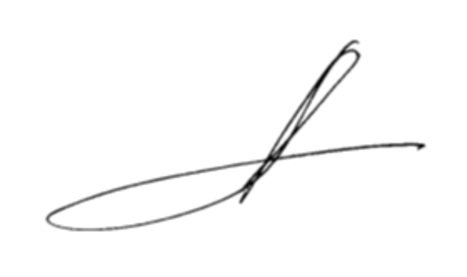
\includegraphics[height=1.7cm]{secretary-signature}
    \end{tabular}
&
    \begin{tabular}{l}
        \sfs \defenseSecretaryFio \\
        \sfs \defenseSecretaryRegalia
    \end{tabular}
\end{tabular}
%\end{table}
\newpage
